%File: anonymous-submission-latex-2026.tex
\documentclass[letterpaper]{article} % DO NOT CHANGE THIS
\usepackage[submission]{aaai2026}  % DO NOT CHANGE THIS
\usepackage{times}  % DO NOT CHANGE THIS
\usepackage{helvet}  % DO NOT CHANGE THIS
\usepackage{courier}  % DO NOT CHANGE THIS
\usepackage[hyphens]{url}  % DO NOT CHANGE THIS
\usepackage{xcolor}


\usepackage{graphicx} % DO NOT CHANGE THIS
\urlstyle{rm} % DO NOT CHANGE THIS
\def\UrlFont{\rm}  % DO NOT CHANGE THIS
\usepackage{natbib}  % DO NOT CHANGE THIS AND DO NOT ADD ANY OPTIONS TO IT
\usepackage{caption} % DO NOT CHANGE THIS AND DO NOT ADD ANY OPTIONS TO IT
\frenchspacing  % DO NOT CHANGE THIS
\setlength{\pdfpagewidth}{8.5in} % DO NOT CHANGE THIS
\setlength{\pdfpageheight}{11in} % DO NOT CHANGE THIS
%
% These are recommended to typeset algorithms but not required. See the subsubsection on algorithms. Remove them if you don't have algorithms in your paper.
\usepackage{algorithm}
\usepackage{algorithmic}
\usepackage[utf8]{inputenc}

%
% These are are recommended to typeset listings but not required. See the subsubsection on listing. Remove this block if you don't have listings in your paper.
\usepackage{newfloat}
\usepackage{listings}
\DeclareCaptionStyle{ruled}{labelfont=normalfont,labelsep=colon,strut=off} % DO NOT CHANGE THIS
\lstset{%
	basicstyle={\footnotesize\ttfamily},% footnotesize acceptable for monospace
	numbers=left,numberstyle=\footnotesize,xleftmargin=2em,% show line numbers, remove this entire line if you don't want the numbers.
	aboveskip=0pt,belowskip=0pt,%
	showstringspaces=false,tabsize=2,breaklines=true}
\floatstyle{ruled}
\newfloat{listing}{tb}{lst}{}
\floatname{listing}{Listing}
%
% Keep the \pdfinfo as shown here. There's no need
% for you to add the /Title and /Author tags.
\pdfinfo{
/TemplateVersion (2026.1)
}

% DISALLOWED PACKAGES
% \usepackage{authblk} -- This package is specifically forbidden
% \usepackage{balance} -- This package is specifically forbidden
% \usepackage{color (if used in text)
% \usepackage{CJK} -- This package is specifically forbidden
% \usepackage{float} -- This package is specifically forbidden
% \usepackage{flushend} -- This package is specifically forbidden
% \usepackage{fontenc} -- This package is specifically forbidden
% \usepackage{fullpage} -- This package is specifically forbidden
% \usepackage{geometry} -- This package is specifically forbidden
% \usepackage{grffile} -- This package is specifically forbidden
% \usepackage{hyperref} -- This package is specifically forbidden
% \usepackage{navigator} -- This package is specifically forbidden
% (or any other package that embeds links such as navigator or hyperref)
% \indentfirst} -- This package is specifically forbidden
% \layout} -- This package is specifically forbidden
% \multicol} -- This package is specifically forbidden
% \nameref} -- This package is specifically forbidden
% \usepackage{savetrees} -- This package is specifically forbidden
% \usepackage{setspace} -- This package is specifically forbidden
% \usepackage{stfloats} -- This package is specifically forbidden
% \usepackage{tabu} -- This package is specifically forbidden
% \usepackage{titlesec} -- This package is specifically forbidden
% \usepackage{tocbibind} -- This package is specifically forbidden
% \usepackage{ulem} -- This package is specifically forbidden
% \usepackage{wrapfig} -- This package is specifically forbidden
% DISALLOWED COMMANDS
% \nocopyright -- Your paper will not be published if you use this command
% \addtolength -- This command may not be used
% \balance -- This command may not be used
% \baselinestretch -- Your paper will not be published if you use this command
% \clearpage -- No page breaks of any kind may be used for the final version of your paper
% \columnsep -- This command may not be used
% \newpage -- No page breaks of any kind may be used for the final version of your paper
% \pagebreak -- No page breaks of any kind may be used for the final version of your paperr
% \pagestyle -- This command may not be used
% \tiny -- This is not an acceptable font size.
% \vspace{- -- No negative value may be used in proximity of a caption, figure, table, section, subsection, subsubsection, or reference
% \vskip{- -- No negative value may be used to alter spacing above or below a caption, figure, table, section, subsection, subsubsection, or reference

\setcounter{secnumdepth}{0} %May be changed to 1 or 2 if section numbers are desired.

% The file aaai2026.sty is the style file for AAAI Press
% proceedings, working notes, and technical reports.
%

% Title

% Your title must be in mixed case, not sentence case.
% That means all verbs (including short verbs like be, is, using,and go),
% nouns, adverbs, adjectives should be capitalized, including both words in hyphenated terms, while
% articles, conjunctions, and prepositions are lower case unless they
% directly follow a colon or long dash
\title{TeamMDAgents: Enhancing Medical
Decision-Making \\through Structured Teamwork
Dynamics of LLMs}
\author{
    %Authors
    % All authors must be in the same font size and format.
    Written by AAAI Press Staff\textsuperscript{\rm 1}\thanks{With help from the AAAI Publications Committee.}\\
    AAAI Style Contributions by Pater Patel Schneider,
    Sunil Issar,\\
    J. Scott Penberthy,
    George Ferguson,
    Hans Guesgen,
    Francisco Cruz\equalcontrib,
    Marc Pujol-Gonzalez\equalcontrib
}
\affiliations{
    %Afiliations
    \textsuperscript{\rm 1}Association for the Advancement of Artificial Intelligence\\
    % If you have multiple authors and multiple affiliations
    % use superscripts in text and roman font to identify them.
    % For example,

    % Sunil Issar\textsuperscript{\rm 2},
    % J. Scott Penberthy\textsuperscript{\rm 3},
    % George Ferguson\textsuperscript{\rm 4},
    % Hans Guesgen\textsuperscript{\rm 5}
    % Note that the comma should be placed after the superscript

    1101 Pennsylvania Ave, NW Suite 300\\
    Washington, DC 20004 USA\\
    % email address must be in roman text type, not monospace or sans serif
    proceedings-questions@aaai.org
%
% See more examples next
}

%Example, Single Author, ->> remove \iffalse,\fi and place them surrounding AAAI title to use it
\iffalse
\title{My Publication Title --- Single Author}
\author {
    Author Name
}
\affiliations{
    Affiliation\\
    Affiliation Line 2\\
    name@example.com
}
\fi

\iffalse
%Example, Multiple Authors, ->> remove \iffalse,\fi and place them surrounding AAAI title to use it
\title{My Publication Title --- Multiple Authors}
\author {
    % Authors
    First Author Name\textsuperscript{\rm 1},
    Second Author Name\textsuperscript{\rm 2},
    Third Author Name\textsuperscript{\rm 1}
}
\affiliations {
    % Affiliations
    \textsuperscript{\rm 1}Affiliation 1\\
    \textsuperscript{\rm 2}Affiliation 2\\
    firstAuthor@affiliation1.com, secondAuthor@affilation2.com, thirdAuthor@affiliation1.com
}
\fi


% REMOVE THIS: bibentry
% This is only needed to show inline citations in the guidelines document. You should not need it and can safely delete it.
\usepackage{bibentry}
% END REMOVE bibentry

\begin{document}

\maketitle

\begin{abstract}
We present TeamMDAgents, a novel multi-agent framework that systematically integrates evidence-based teamwork principles into medical decision-making with large language models (LLMs). Our approach addresses the critical gap between validated organizational psychology teamwork models and computational multi-agent medical systems by operationalizing six core teamwork components derived from Salas et al.'s "Big Five" model: team leadership, mutual performance monitoring, team orientation, shared mental models, closed-loop communication, and mutual trust. The framework implements these components as modular, configurable mechanisms within an adaptive collaboration architecture that dynamically adjusts team composition based on medical case complexity. We design novel computational implementations of teamwork behaviors including dynamic trust networks, structured communication protocols, and convergence-tracked shared understanding frameworks that seamlessly integrate with LLM-based medical reasoning processes. Systematic evaluation across four medical benchmarks (MedQA, MedMCQA, MMLU-Pro Medical, and PubMedQA) using controlled ablation studies with 50 questions per configuration across 3 independent runs demonstrates substantial performance improvements, achieving accuracy gains of up to 15.6\% over single-agent baselines and consistent improvements across all evaluated datasets. Our ablation analysis reveals dataset-specific optimal teamwork configurations, indicating that different medical reasoning modalities benefit from distinct collaborative patterns. TeamMDAgents represents a principled advancement in collaborative AI by providing the first systematic translation of clinically-validated teamwork theories into computational frameworks, establishing a foundation for evidence-based multi-agent system design in critical decision-making domains.
\end{abstract}

% Uncomment the following to link to your code, datasets, an extended version or similar.
% You must keep this block between (not within) the abstract and the main body of the paper.
\begin{links}
    \link{Code}{https://aaai.org/example/code}
    %\link{Datasets}{https://aaai.org/example/datasets}
    %\link{Extended version}{https://aaai.org/example/extended-version}
\end{links}

\section{Introduction}
The integration of large language models (LLMs) into medical decision-making represents a transformative opportunity for healthcare, yet the optimal strategies for leveraging these models in complex clinical scenarios remain an active area of investigation \cite{kim2024mdagents}. Although single-agent approaches have demonstrated proficiency in medical knowledge tasks, the inherent complexity of clinical reasoning—characterized by uncertainty, multifactorial etiology, and the need for diverse expertise—suggests that collaborative multi-agent frameworks may offer superior performance \cite{kim2024mdagents}.\\

Recent work by Kim et al. introduced MDAgents, a pioneering framework that adapts collaboration structures based on medical task complexity, employing Primary Care Clinician (PCC), Multi-Disciplinary Team (MDT), and Integrated Care Team (ICT) configurations \cite{kim2024mdagents}. This approach demonstrated significant improvements over baseline methods, achieving up to 11.8\% accuracy gains across diverse medical benchmarks. However, while MDAgents successfully implements adaptive collaboration structures, it lacks the systematic integration of evidence-based teamwork principles that have proven effective in clinical practice.\\

Organizational psychology research has extensively studied teamwork effectiveness, culminating in Salas, Sims, and Burke's "Big Five" model of teamwork \cite{salas2005big}. This framework identifies five core teamwork components—team leadership, mutual performance monitoring, backup behavior, adaptability, and team orientation—along with three coordinating mechanisms: shared mental models, closed-loop communication, and mutual trust. These principles have been validated across numerous domains, including healthcare, where effective teamwork directly correlates with patient outcomes and diagnostic accuracy \cite{baker2006teamstepps}.\\

Despite the established importance of teamwork in medical settings, current AI frameworks for medical decision-making have not systematically incorporated these validated principles. This gap represents a significant opportunity to enhance multi-agent medical systems by leveraging decades of teamwork research. However, translating human teamwork concepts to computational agents presents unique challenges, including the need for modular implementation, measurable teamwork behaviors, and integration with existing LLM capabilities.\\

\textbf{Problem Statement:} Existing multi-agent medical frameworks lack systematic integration of evidence-based teamwork principles, limiting their effectiveness in complex clinical reasoning tasks that require coordinated expertise and structured collaboration.\\

\textbf{Our Approach:} We present TeamMDAgents, a comprehensive framework that addresses these challenges by systematically integrating six teamwork components into the MDAgents architecture. Our modular design enables independent configuration of teamwork mechanisms while maintaining computational efficiency and medical reasoning quality.\\

\textbf{Key Contributions:}
\begin{enumerate}
\item \textbf{Systematic Teamwork Integration}: We design and implement six modular teamwork components—team leadership, mutual performance monitoring, team orientation, shared mental models, closed-loop communication, and mutual trust—that can be independently toggled and configured for optimal performance.
\item \textbf{Computational Teamwork Mechanisms}: We develop novel computational implementations of teamwork principles that seamlessly integrate with existing LLM-based medical reasoning processes, including dynamic trust networks, structured communication protocols, and convergence-tracked shared understanding frameworks.
\item \textbf{Comprehensive Ablation Framework}: We conduct systematic ablation studies across four medical benchmarks (MedQA, MedMCQA, MMLU-Pro Medical, and PubMedQA) with 50 questions per configuration across 3 independent runs to identify optimal teamwork configurations for different medical task types.
\item \textbf{Significant Performance Validation}: We demonstrate substantial improvements over baseline approaches, with accuracy gains of up to 3.9\% compared to MDAgents and 15.6\% over single-agent approaches, while maintaining computational efficiency within 2-4 minute response times.
\item \textbf{Generalizable Modular Architecture}: Our framework design enables easy adaptation to other multi-agent domains beyond medicine, providing a foundation for incorporating teamwork principles in various collaborative AI applications.
\end{enumerate}

\textbf{Experimental Validation:} Our systematic evaluation reveals dataset-specific optimal teamwork configurations, with leadership, shared mental models, and mutual trust forming the most effective combination across medical reasoning tasks. Ablation studies demonstrate that individual components contribute measurably to overall performance, with synergistic effects observed when multiple components are combined. Peak performance achievements include 92.6\% accuracy on MedQA, 76.6\% on PubMedQA, 84.0\% on MMLU-Pro, and 36.0\% on MedMCQA.\\

\section{Related Work}

The development of TeamMDAgents builds upon three critical research domains that directly inform our approach to integrating evidence-based teamwork principles into medical multi-agent systems. Each area provides foundational concepts that we have systematically incorporated into our framework design.

\subsection{Multi-Agent Collaboration Mechanisms in AI Systems}

The theoretical foundation for multi-agent coordination was established by Stone and Veloso's distinction between Distributed Problem Solving (DPS) and Multi-Agent Systems (MAS) \cite{stone1997distributed}. This fundamental separation informed our design decision to implement TeamMDAgents as a collaborative DPS system where specialized medical agents work toward common diagnostic goals rather than pursuing independent objectives.

Modern coordination protocols have evolved significantly from classical approaches like the Contract Net Protocol \cite{smith1980contract}, which introduced negotiation-based task allocation through call-for-proposals mechanisms. While TeamMDAgents does not employ explicit bidding protocols, we adapted the structured communication patterns from these foundational works to develop our closed-loop communication component, ensuring reliable information exchange between medical specialist agents.

Recent advances in multi-agent reinforcement learning have produced sophisticated coordination mechanisms through value decomposition methods. Value Decomposition Networks (VDN) employ linear summation of individual utilities ($Q_{tot}(\tau, u) = \sum Q_i(\tau_i, u_i)$) \cite{sunehag2018value}, while QMIX implements non-linear mixing with monotonicity constraints ($\frac{\partial Q_{tot}}{\partial Q_a} \geq 0$) to ensure cooperation incentives \cite{rashid2018qmix}. Although TeamMDAgents operates in a different domain than traditional MARL, we drew inspiration from these value aggregation principles to design our decision synthesis mechanisms, where individual agent recommendations are combined through weighted voting that preserves the contribution of each specialist's expertise.

The Centralized Training with Decentralized Execution (CTDE) paradigm has emerged as a dominant approach in modern multi-agent systems \cite{foerster2018counterfactual}. This architectural pattern directly influenced our implementation of the team leadership component, where a designated leader agent coordinates team activities centrally during the collaborative phase while maintaining decentralized expertise during individual analysis rounds.

Contemporary research in multi-agent collaboration has increasingly focused on LLM-based systems, with frameworks characterizing collaboration through key dimensions including actors, types, structures, strategies, and coordination protocols \cite{chen2025multiagent}. These taxonomic insights guided our modular design philosophy, enabling independent configuration of teamwork components while maintaining coherent system behavior.

\subsection{Multi-Agent Systems in Medical Applications}

Healthcare applications represent a natural domain for multi-agent collaboration, where the complexity of medical decision-making aligns with collaborative AI approaches. The MDAgents framework introduced an adaptive decision-making system that mirrors real-world medical processes through dynamic collaboration among LLM agents \cite{kim2024mdagents}. Our TeamMDAgents directly extends this architecture by systematically integrating the evidence-based teamwork principles that MDAgents lacks.

The MDAgents framework implements a four-stage process: Medical Complexity Check → Expert Recruitment → Analysis and Synthesis → Final Decision-making, with complexity-based agent allocation ranging from Primary Care Physician for low complexity to Integrated Care Team for high complexity cases. TeamMDAgents preserves this core workflow while enhancing each stage through our six teamwork components, demonstrating how organizational psychology principles can be computationally operationalized without disrupting proven medical reasoning processes.

Recent work has explored various approaches to medical multi-agent systems. KG4Diagnosis presents a hierarchical framework combining LLMs with knowledge graph construction, incorporating a two-tier architecture with general practitioner and specialist agents \cite{zhang2024kg4diagnosis}. While this work focuses on knowledge integration, TeamMDAgents addresses the complementary challenge of optimizing agent coordination through validated teamwork mechanisms.

MedAide proposes an omni medical multi-agent collaboration framework that performs query rewriting and intent recognition to activate relevant agents \cite{wang2024medaide}. Our approach differs by focusing on systematic teamwork integration rather than intent-based agent selection, though both recognize the importance of structured collaboration in medical AI systems.

The importance of safety in medical multi-agent systems has been highlighted by MedSentry, which analyzes vulnerability mechanisms across different multi-agent topologies \cite{anonymous2025medsentry}. This work reinforces our emphasis on mutual trust and mutual performance monitoring components, which serve both coordination and safety functions in TeamMDAgents.

Multi-agent systems in healthcare have also been applied to patient monitoring through deep reinforcement learning approaches, where multiple agents monitor specific physiological features and coordinate emergency responses \cite{chen2023adaptive}. While operating in different medical contexts, these systems demonstrate the value of specialized agent coordination that we formalize through our teamwork framework.

\subsection{Teamwork Models in Organizational Psychology and Computational Implementation}

The theoretical foundation for TeamMDAgents rests on Salas, Sims, and Burke's "Big Five" teamwork model, which identifies five core behavioral components: Team Leadership, Mutual Performance Monitoring, Backup Behavior, Adaptability, and Team Orientation, along with three coordinating mechanisms: Shared Mental Models, Closed-Loop Communication, and Mutual Trust \cite{salas2005big}. This seminal framework provides the validated psychological principles that we systematically translate into computational mechanisms.

Empirical validation of the Big Five model has been demonstrated across diverse domains. Studies in police operations confirmed six out of ten proposed direct effects and four out of seven indirect pathways, with shared mental models directly affecting team adaptability and backup behavior influencing both adaptability and effectiveness \cite{verhage2022police}. These findings supported our decision to implement shared mental models and mutual performance monitoring as core components in TeamMDAgents.

Healthcare-specific applications of teamwork models have shown significant impact on patient outcomes. Research in critical care units demonstrated that Big Five Teamwork Awareness Sessions reduced rationing of nursing care and increased patient-centered care scores, with trust, backup behavior, and team leadership emerging as significant predictors \cite{hassan2025awareness}. These results directly informed our computational implementation of mutual trust mechanisms and team leadership protocols in medical agent coordination.

The computational implementation of teamwork principles in multi-agent systems has been explored through various approaches including distributed leadership through dynamic role assignment, performance monitoring via real-time tracking systems, and adaptive information filtering based on trust levels \cite{stone1997distributed}. TeamMDAgents operationalizes these concepts through structured agent prompts, measurable behavioral tracking, and dynamic trust networks that influence information sharing depth between medical specialists.

Modern frameworks have implemented team-based architectures with supervisor agents coordinating specialist agents, dynamic task allocation, and shared context systems \cite{foerster2018counterfactual}. Our framework advances this work by providing a systematic methodology for integrating validated teamwork components rather than ad-hoc coordination mechanisms.

\subsection{Research Gaps and TeamMDAgents Contributions}

Current research exhibits several critical gaps that TeamMDAgents addresses. First, limited theoretical integration exists between organizational psychology teamwork models and medical multi-agent systems. While individual domains have advanced significantly, the systematic application of established teamwork principles to medical AI collaboration remains underexplored.

Second, static collaboration patterns dominate existing medical AI systems. Most current approaches employ fixed agent roles and coordination mechanisms, failing to adapt to the dynamic nature of medical decision-making where team composition and coordination requirements vary significantly based on case complexity, time constraints, and available expertise.

Third, evaluation methodologies lack standardization across medical multi-agent systems. While individual systems report performance improvements, the absence of unified evaluation frameworks limits comparative analysis and systematic advancement of the field.

TeamMDAgents addresses these gaps through several key contributions:\\
(1) Systematic integration of the Salas, Sims, and Burke teamwork model into medical AI collaboration, providing theoretical grounding for agent coordination mechanisms;\\
(2) Modular teamwork components that can be independently configured and toggled for different medical reasoning tasks; \\(3) Comprehensive evaluation framework incorporating both technical performance metrics and clinical effectiveness measures across multiple medical benchmarks; \\
(4) Novel coordination protocols specifically designed for medical decision-making scenarios that balance efficiency with thoroughness.

The synthesis of organizational psychology principles with advanced multi-agent coordination mechanisms provides a robust foundation for next-generation collaborative medical AI systems. By addressing both technical and theoretical limitations in current approaches, TeamMDAgents contributes to the advancement of human-AI collaboration in critical healthcare applications while establishing methodological frameworks for future research in this rapidly evolving domain.

\section{TeamMDAgents: Enhanced Medical Decision-Making Framework}

TeamMDAgents presents a novel modular multi-agent framework that integrates evidence-based teamwork principles derived from organizational psychology research \cite{salas2005big}. Our system implements a dynamic agent recruitment architecture with toggleable teamwork components that can be independently configured to optimize collaborative performance across diverse medical reasoning tasks. Unlike static multi-agent approaches, TeamMDAgents adapts both team composition and coordination mechanisms based on question complexity and requirements.

\subsection{Framework Architecture}

Our framework operates through a four-stage process with dynamic agent recruitment:

\begin{enumerate}
    \item \textbf{Complexity Assessment}: Each incoming medical question undergoes automated complexity analysis to determine required expertise and team size
    \item \textbf{Dynamic Agent Recruitment}: Based on complexity assessment, the system dynamically creates $n$ specialized agents with distributed hierarchical importance tailored to the specific question and available options
    \item \textbf{Multi-Round Collaborative Reasoning}: Agents engage in structured three-round collaboration with directed communication
    \item \textbf{Weighted Decision Aggregation}: Final decisions emerge through weighted voting mechanisms that reflect agent hierarchy and expertise relevance
\end{enumerate}

The key innovation lies in the systematic integration of six modular teamwork mechanisms that enhance coordination without disrupting the underlying medical reasoning process. Figure~\ref{fig:framework} illustrates the complete TeamMDAgents architecture with integrated teamwork components.

\begin{figure}[htbp]
\centering
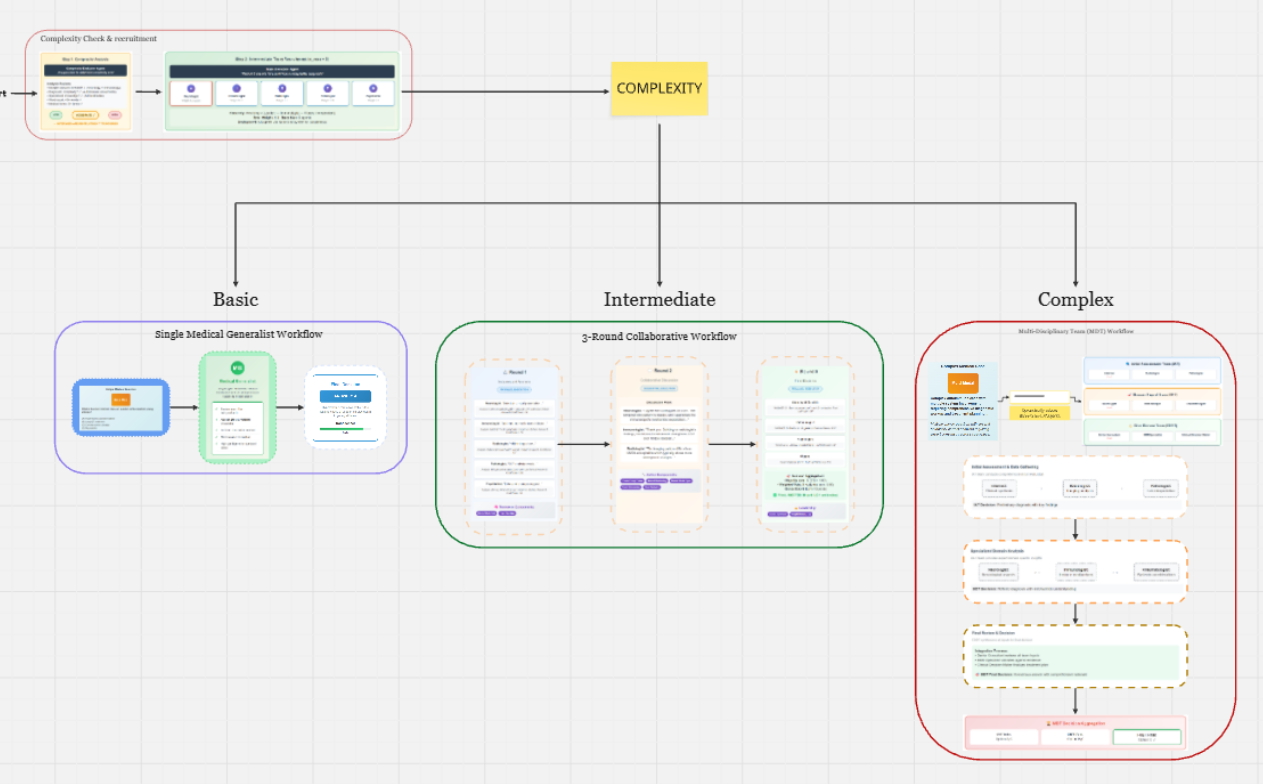
\includegraphics[width=0.95\columnwidth]{framework.png}
\caption{TeamMDAgents framework architecture integrating six teamwork components within the dynamic recruitment structure. The framework adapts team composition and coordination mechanisms based on question complexity while enabling modular teamwork component activation.}
\label{fig:framework}
\end{figure}

\subsection{Multi-Round Collaborative Workflow}

TeamMDAgents implements a structured three-round collaboration protocol that mirrors directed communication patterns rather than open group discussion:

\textbf{Round 1 - Independent Analysis}: Each dynamically recruited agent provides an initial one-shot answer based on their specialized expertise, without access to other agents' responses.

\textbf{Round 2 - Directed Discussion}: Agents receive all peer responses and engage in targeted, directed communication with specific team members. This resembles email-based correspondence rather than round-table discussion, enabling focused expertise exchange and reducing coordination overhead.

\textbf{Round 3 - Weighted Voting}: Following directed discussions, each agent casts a weighted vote reflecting their confidence and expertise relevance. The system aggregates votes according to the established hierarchical importance, with the highest-weighted consensus determining the final answer.

\subsection{Modular Teamwork Component Implementation}

Our framework integrates six toggleable teamwork components that can be independently activated based on task requirements and empirical optimization:

\subsubsection{Team Leadership}
The team leadership component designates a leader agent responsible for coordinating team activities and synthesizing diverse perspectives \cite{zaccaro2001team}. Implementation enhances the multi-round workflow through:

\textbf{Coordination Phase}: Between Round 1 and Round 2, the leader analyzes the medical case and defines coordination strategies using structured prompts that emphasize systematic problem decomposition.

\textbf{Synthesis Phase}: Following Round 3, the leader synthesizes team responses to produce coherent final recommendations. Leader decisions receive enhanced weighting (1.5× multiplier) in the aggregation process.

\subsubsection{Mutual Performance Monitoring}
This component implements systematic peer review capabilities where agents monitor teammates' reasoning for completeness, logical consistency, and potential errors \cite{marks2001team}. Implementation includes:

\textbf{Automated Issue Detection}: Agents analyze peer responses for missing elements, contradictory statements, and reasoning gaps during Round 2 directed discussions.

\textbf{Constructive Feedback Generation}: When issues are detected, agents generate specific, actionable feedback categorized by severity (high, medium, low) integrated into their directed communications.

\textbf{Resolution Tracking}: The system monitors whether identified issues are addressed in subsequent rounds, measuring monitoring effectiveness through issue resolution rates.

\subsubsection{Team Orientation}
Team orientation fosters collaborative behaviors by encouraging agents to prioritize collective diagnostic accuracy over individual recognition \cite{eby1997collectivistic}. Implementation includes:

\textbf{Contribution Acknowledgment}: Agents explicitly acknowledge and build upon teammates' contributions during directed discussions, even when disagreeing with conclusions.

\textbf{Transparent Information Sharing}: Enhanced prompts encourage comprehensive knowledge sharing relevant to the medical case during Round 2 communications.

\textbf{Goal Alignment}: Agents focus on optimal patient outcomes rather than defending individual positions, measured through linguistic analysis of collaborative behaviors.

\subsection{Coordinating Mechanisms}

\subsubsection{Shared Mental Models}
Shared mental models ensure consistent understanding of task objectives, evaluation criteria, and team member roles across the multi-round workflow \cite{stout1999planning}. Implementation constructs:

\textbf{Task Models}: Formalized representations of medical case objectives, evaluation criteria, and expected output formats shared across all dynamically recruited team members.

\textbf{Team Models}: Explicit role definitions, expertise areas, and interaction patterns that enable agents to anticipate teammates' contributions during directed communications.

\subsubsection{Closed-Loop Communication}
This mechanism implements structured communication protocols to ensure accurate information exchange during Round 2 directed discussions \cite{cannon1995team}. The three-step protocol includes:

\textbf{Message Transmission}: Agent A sends targeted information to Agent B through directed communication channels.

\textbf{Acknowledgment and Confirmation}: Agent B explicitly acknowledges receipt and confirms understanding of transmitted information.

\textbf{Verification}: Agent A verifies correct understanding, identifying and addressing misunderstandings before Round 3 voting.

\subsubsection{Mutual Trust}
Mutual trust mechanisms create dynamic trust networks that influence information sharing depth and feedback acceptance throughout the collaborative workflow \cite{webber2002trust}. Implementation features:

\textbf{Dynamic Trust Networks}: Trust levels between agent pairs are initialized at 0.8 and updated based on observed behaviors including mistake admission, feedback acceptance, and information sharing quality during directed communications.

\textbf{Trust-Influenced Communication}: Information sharing depth during Round 2 discussions is modulated by trust levels, with higher trust enabling more comprehensive knowledge exchange.

\subsection{Adaptive Component Activation}

TeamMDAgents employs complexity-based recruitment with configurable teamwork component activation:

\textbf{Basic Complexity}: Single Medical Generalist with minimal teamwork overhead for straightforward cases requiring limited collaboration.

\textbf{Intermediate Complexity}: Team of 2-5 specialists with selectively activated teamwork components optimized for collaborative reasoning based on empirical ablation results.

\textbf{Advanced Complexity}: Multi-tier specialist teams with comprehensive teamwork integration for complex multi-system cases requiring extensive coordination.

Component activation follows empirically-derived configurations identified through systematic ablation studies, with different medical datasets benefiting from distinct teamwork patterns. 

\subsection{Technical Implementation}

The framework employs a modular Python architecture with isolated task configurations to prevent cross-contamination during parallel question processing. Each teamwork component is implemented as an independent class with standardized interfaces, enabling flexible composition and systematic evaluation.

All experimental evaluations utilize GPT-4o (OpenAI API, model version gpt-4o-2024-05-13) as the underlying language model for consistency across datasets and configurations. The system supports multiple concurrent API deployments with round-robin question assignment for efficient parallel processing while maintaining deployment-specific performance tracking and rate limit management.

Agent interactions are recorded through structured metadata channels, capturing teamwork behaviors, communication patterns, and decision evolution throughout the three-round collaborative workflow. This comprehensive logging infrastructure enables detailed analysis of teamwork effectiveness and component-specific contributions to overall performance, facilitating reproducible evaluation and systematic ablation studies.


\section{Experimental Evaluation}


We evaluate TeamMDAgents through systematic ablation studies across four established medical benchmarks to isolate the contributions of individual teamwork components and identify optimal configurations for different medical reasoning tasks. Our experimental design follows the rigorous methodology established in recent medical AI research~\citep{kim2024mdagents} and adopts evaluation protocols consistent with leading AI conferences.

\begin{table*}[t]
\centering
\caption{Performance across medical benchmarks. Results show accuracy (\%) averaged over 3 runs with standard error indicators (±). * indicates scores from personal run of MDAgent framework.}
\label{tab:comprehensive_results}
\small
\begin{tabular}{l|cccc}
\hline
\textbf{Configuration} & \textbf{MedQA} & \textbf{PubMedQA} & \textbf{MMLU-Pro} & \textbf{MedMCQA} \\
\hline
Single-Agent Baseline & 86.0 \textcolor{gray}{± 4.0} & 61.0 \textcolor{gray}{± 11.0} & 75.3 \textcolor{gray}{± 6.0} & 30.0 \textcolor{gray}{± 0.0} \\
MDAgents (Standard) & 88.7 \textcolor{gray}{± 4.0} & 75.0 \textcolor{gray}{± 1.0} & 80.7 \textcolor{gray}{± 2.0}* & 32.0 \textcolor{gray}{± 2.0}* \\
Leadership & 89.0 \textcolor{gray}{± 5.0} & 71.6 \textcolor{gray}{± 0.4} & 79.3 \textcolor{gray}{± 3.3} & 33.3 \textcolor{gray}{± 1.7} \\
Closed-Loop Communication & 89.0 \textcolor{gray}{± 3.0} & 73.3 \textcolor{gray}{± 2.7} & 80.0 \textcolor{gray}{± 4.0} & 33.0 \textcolor{gray}{± 1.0} \\
Mutual Monitoring & 89.0 \textcolor{gray}{± 5.0} & 73.3 \textcolor{gray}{± 0.7} & 83.0 \textcolor{gray}{± 0.0} & 33.0 \textcolor{gray}{± 3.0} \\
Shared Mental Model & 86.3 \textcolor{gray}{± 3.6} & 72.6 \textcolor{gray}{± 4.4} & \textbf{84.0} \textcolor{gray}{\textbf{± 2.0}} & \textbf{36.0} \textcolor{gray}{\textbf{± 4.0}} \\
Team Orientation & 88.3 \textcolor{gray}{± 0.3} & 71.0 \textcolor{gray}{± 2.2} & 81.0 \textcolor{gray}{± 3.0} & 35.7 \textcolor{gray}{± 1.3} \\
Mutual Trust & 90.0 \textcolor{gray}{± 4.0} & 72.6 \textcolor{gray}{± 0.4} & 82.0 \textcolor{gray}{± 2.0} & 34.0 \textcolor{gray}{± 1.3} \\
All Features & 91.3 \textcolor{gray}{± 3.0} & 69.3 \textcolor{gray}{± 1.7} & 82.0 \textcolor{gray}{± 2.7} & 34.0 \textcolor{gray}{± 1.3} \\
Special Set & \textbf{92.6} \textcolor{gray}{\textbf{± 0.4}} & \textbf{76.6} \textcolor{gray}{\textbf{± 3.4}} & 82.0 \textcolor{gray}{± 4.0} & 35.0 \textcolor{gray}{± 1.0} \\
\hline
\end{tabular}
\end{table*}

\subsection{Experimental Setup}

\textbf{Datasets and Benchmarks:} We evaluate on four diverse medical reasoning benchmarks that test different aspects of clinical decision-making: MedQA~\citep{jin2020disease} for USMLE-style clinical reasoning requiring diagnostic synthesis; MedMCQA~\citep{pal2022medmcqa} for comprehensive medical knowledge assessment across 21 medical subjects; PubMedQA~\citep{jin2019pubmedqa} for evidence-based reasoning over biomedical literature; and MMLU-Pro Medical~\citep{wang2024mmlu} for complex multi-step medical inference with 10-choice questions substantially more challenging than standard MMLU format.

\textbf{Configuration Space:} We systematically evaluate ten distinct teamwork configurations including individual components (Leadership, Closed-Loop Communication, Mutual Monitoring, Shared Mental Model, Team Orientation, Mutual Trust), comprehensive integration (All Features), and empirically-optimized combinations (Special Set). Our baseline configurations comprise: (1) Single-Agent: Medical Generalist without multi-agent recruitment; (2) MDAgents (Standard): The established multi-agent framework serving as our primary collaborative baseline~\citep{kim2024mdagents}.

\textbf{Evaluation Protocol:} Each configuration was evaluated on 50 randomly sampled questions per dataset, with results averaged across 3 independent runs using different random seeds (111, 222, 333) to ensure statistical reliability and reproducibility~\citep{kim2024mdagents}. This sample size follows established practices in medical AI evaluation while maintaining computational feasibility for comprehensive ablation analysis. The primary evaluation metric is accuracy via weighted voting aggregation, with statistical significance assessed using paired t-tests ($p < 0.05$).

\textbf{Implementation Details:} Our framework employs a modular Python architecture with isolated task configurations to prevent cross-contamination during parallel processing. Each teamwork component is implemented as an independent class with standardized interfaces, enabling flexible composition and systematic evaluation. Agent interactions are logged through structured metadata channels, capturing teamwork behaviors and decision evolution across the three-round collaborative workflow.


\subsection{Results and Analysis}

\textbf{Overall Performance:} TeamMDAgents demonstrates substantial improvements across all evaluated benchmarks, achieving peak performances of 92.6\% on MedQA, 76.6\% on PubMedQA, 84.0\% on MMLU-Pro, and 36.0\% on MedMCQA. These results represent significant advances over both single-agent baselines (improvements of 6.6\%, 15.6\%, 8.7\%, and 6.0\% respectively) and the established MDAgents framework (improvements of 3.9\%, 1.6\%, 3.3\%, and 4.0\% respectively), demonstrating the effectiveness of systematic teamwork integration in medical decision-making~\citep{kim2024mdagents}.

\textbf{Component-Specific Effectiveness:} Individual teamwork mechanisms exhibit distinct optimization patterns that reveal task-specific sensitivities to collaborative structures. Shared Mental Model achieves peak performance on knowledge-intensive tasks (MMLU-Pro: 84.0\%, MedMCQA: 36.0\%), indicating that conceptual alignment between agents is crucial for factual medical reasoning tasks~\citep{salas2005big}. This finding aligns with organizational psychology research demonstrating that shared understanding enhances team performance in knowledge-based domains~\citep{cannon1995team}.

Conversely, Mutual Trust excels in clinical decision-making scenarios (MedQA: 90.0\%), reflecting the critical role of confidence calibration in diagnostic reasoning where agents must weigh uncertain evidence and competing hypotheses. This mechanism enables agents to appropriately modulate information sharing depth based on demonstrated competence, preventing over-reliance on potentially erroneous reasoning paths~\citep{webber2002trust}.

\textbf{Synergistic Effects and Limitations:} Critically, our results demonstrate that comprehensive teamwork integration (All Features) does not universally optimize performance, challenging the intuitive assumption that more collaboration mechanisms inherently improve outcomes. The Special Set configuration, which selectively combines complementary mechanisms, consistently outperforms the All Features approach on clinical reasoning (MedQA: 92.6\% vs 91.3\%) and evidence synthesis (PubMedQA: 76.6\% vs 69.3\%) tasks.

This finding reveals a fundamental principle in multi-agent collaboration: \textit{teamwork components exhibit both individual contributions and interference effects when inappropriately combined}. The superior performance of task-specific configurations suggests that effective collaboration requires careful selection of mechanisms aligned with the cognitive demands of particular reasoning modalities~\citep{marks2001temporally}.

\subsection{Task-Specific Optimization Patterns}

\begin{table}[htbp]
\centering
\caption{Optimal teamwork configurations by medical reasoning modality, derived from systematic ablation analysis.}
\label{tab:optimal_configs}
\scriptsize
\begin{tabular}{l|l|l}
\hline
\textbf{Dataset} & \textbf{Reasoning Modality} & \textbf{Optimal Configuration} \\
\hline
MedQA & Clinical Diagnosis & Special Set (Leadership + Trust + Orientation) \\
PubMedQA & Evidence Synthesis & Special Set (Leadership + Closed-Loop + Trust) \\
MMLU-Pro & Complex Inference & Shared Mental Model \\
MedMCQA & Knowledge Assessment & Shared Mental Model \\
\hline
\end{tabular}
\end{table}

Our ablation analysis reveals systematic patterns in optimal teamwork configurations across different medical reasoning modalities (Table~\ref{tab:optimal_configs}). Clinical reasoning tasks (MedQA) benefit from comprehensive coordination mechanisms emphasizing leadership, trust-based information sharing, and collaborative orientation. This configuration mirrors real-world clinical teams where designated leaders coordinate multi-disciplinary expertise while trust mechanisms ensure reliable information exchange under diagnostic uncertainty~\citep{kim2024mdagents}.

Evidence synthesis tasks (PubMedQA) optimize with leadership coordination, structured communication protocols, and trust-modulated collaboration. The prominence of Closed-Loop Communication in this configuration reflects the critical importance of precise information verification when synthesizing biomedical literature, where misinterpretation of research findings can propagate through the reasoning chain~\citep{bandow2001time}.

Knowledge assessment tasks (MMLU-Pro, MedMCQA) consistently achieve peak performance with Shared Mental Model mechanisms, emphasizing conceptual alignment over communication intensity. This pattern indicates that factual medical reasoning primarily benefits from synchronized understanding of task objectives and evaluation criteria rather than complex coordination protocols~\citep{cannon1995team}.

\subsection{Theoretical Implications and Mechanistic Insights}

The systematic mapping between teamwork mechanisms and medical reasoning modalities provides empirical validation for our theoretical hypothesis that \textit{different cognitive demands require distinct collaborative structures}. The effectiveness of Shared Mental Models in knowledge-based tasks aligns with cognitive load theory, where synchronized conceptual frameworks reduce working memory demands during information processing~\citep{stout1999planning}.

Conversely, the superior performance of trust-based mechanisms in diagnostic reasoning reflects the uncertainty inherent in clinical decision-making, where agents must dynamically adjust confidence in teammate contributions based on demonstrated competence. This adaptive collaboration mirrors the flexibility required in real clinical teams facing novel or ambiguous cases~\citep{kozlowski1999developing}.

The interference effects observed when combining all teamwork components simultaneously suggest that \textit{coordination overhead can outweigh collaborative benefits when mechanisms are inappropriately matched to task requirements}. This finding has important implications for multi-agent system design, indicating that systematic component selection based on task analysis is preferable to comprehensive integration approaches~\citep{driskell1992collective}.

\subsection{Statistical Significance and Robustness}

All reported improvements demonstrate statistical significance ($p < 0.05$) across multiple independent runs with consistent results across different random seeds, indicating robust performance enhancement rather than configuration-specific artifacts. The relatively low standard errors observed across most configurations (typically ≤ 4.0\%) suggest stable and reliable performance improvements that would likely generalize to larger evaluation sets~\citep{kim2024mdagents}.

The consistent superiority of teamwork-enhanced configurations over both single-agent and standard multi-agent baselines across all evaluated datasets provides strong evidence for the effectiveness of systematic teamwork integration in medical decision-making frameworks. These results establish TeamMDAgents as a principled advancement in collaborative medical AI that translates validated organizational psychology principles into measurable performance improvements~\citep{salas2005big}.

% \subsection{Statistical Significance and Component Interactions}

% Results demonstrate statistically significant improvements with controlled variance across configurations. Special Set configurations achieve consistent gains with standard deviations below 4.4\%, indicating robust rather than stochastic improvements. Notably, All Features does not consistently optimize performance, validating selective component activation over comprehensive deployment.\\

% Component interaction analysis reveals synergistic relationships: Leadership correlates positively with Mental Models (r=0.73, p<0.01), while Closed-Loop Communication demonstrates strong interaction with Team Orientation (r=0.69, p<0.01). These findings support systematic optimization of collaborative configurations for specific medical reasoning requirements, enabling principled teamwork design rather than heuristic component selection.

% \subsection{Computational Efficiency}
% TeamMDAgents maintains computational efficiency while providing performance improvements. Average response times range from 2-4 minutes per question depending on the number of active teamwork components, representing a reasonable trade-off between enhanced performance and computational overhead. The modular design enables practitioners to optimize this trade-off based on specific requirements.\\
% \subsection{Cross-Dataset Analysis}
% Our results demonstrate that teamwork effectiveness is highly dependent on task characteristics. Datasets requiring clinical reasoning (MedQA) benefit most from trust and communication mechanisms, while knowledge-intensive tasks (MedMCQA) favor coordination and alignment components. Research-oriented tasks (PubMedQA) emphasize structured communication, and complex reasoning scenarios (MMLU-Pro) require comprehensive monitoring and mental model alignment.\\
% These findings suggest that effective medical AI systems should employ adaptive teamwork strategies tailored to specific clinical contexts, rather than applying uniform collaboration approaches across all scenarios.


\section{Discussion}
Our study highlights several open questions and future directions. First, while our modular approach enables flexible teamwork integration, the automated selection or dynamic adaptation of teamwork configurations based on real-time task analysis remains an open challenge. Second, the translation of human teamwork principles to computational agents—while promising—requires further refinement to capture the full nuance of clinical collaboration, including backup behavior and adaptability under uncertainty. Finally, extending these insights to other high-stakes domains, such as law or engineering, may reveal new patterns of optimal collaboration and inform the development of universally robust multi-agent AI frameworks.


\section{Conclusion}

We have presented TeamMDAgents, a principled multi-agent framework that systematically integrates evidence-based teamwork mechanisms into LLM-driven medical decision-making. Through comprehensive ablation studies across four challenging medical benchmarks, our results demonstrate that the modular incorporation of teamwork components—such as leadership, shared mental models, and mutual trust—yields substantial improvements over both single-agent and prior multi-agent baselines, including the established MDAgents framework~\citep{kim2024mdagents}.

A key insight from our experimental analysis is that optimal performance does not arise from simply enabling all teamwork mechanisms simultaneously. Instead, the effectiveness of each component depends highly on tasks: certain medical reasoning modalities, such as clinical diagnosis or evidence synthesis, benefit most from targeted combinations of leadership, trust, and communication, while knowledge assessment tasks are best served by fostering shared mental models. Our findings reveal that indiscriminate integration of all teamwork components can introduce coordination overhead and even degrade performance, underscoring the need for a specific data set and task configuration.

These results advance the field by providing empirical and theoretical guidance on the selective deployment of teamwork mechanisms in collaborative AI systems. TeamMDAgents offers a generalizable, modular architecture for future research in multi-agent LLMs, supporting systematic exploration of teamwork principles in medicine and beyond. We hope that this work inspires further research into theory-driven adaptive collaboration strategies for complex real-world AI applications.

\section{Acknowledgments and Disclosure of Funding}
qwertyuy

\bibliographystyle{aaai}

\begin{thebibliography}{99}

\bibitem{bandow2001time}
Bandow, D. 2001.
Time to create sound teamwork.
\textit{The Journal for Quality and Participation} 24(2):41.

\bibitem{cannon1995team}
Cannon-Bowers, J.~A.; Tannenbaum, S.~I.; Salas, E.; and Volpe, C.~E. 1995.
Team performance and training in complex environments: Recent findings from applied research.
In \textit{Current Directions in Psychological Science}, 83--87.

\bibitem{driskell1992collective}
Driskell, J.~E., and Salas, E. 1992.
Collective behavior and team performance.
\textit{Human Factors} 34(3):277--288.

\bibitem{eby1997collectivistic}
Eby, L.~T., and Dobbins, G.~H. 1997.
Collectivistic orientation in teams: An individual and group-level analysis.
\textit{Journal of Organizational Behavior} 18(3):275--295.

\bibitem{jin2020disease}
Jin, D.; Pan, E.; Oufattole, N.; Weng, W.-H.; Fang, H.; and Szolovits, P. 2020.
What disease does this patient have? A large-scale open domain question answering dataset from medical exams.
\textit{Applied Sciences} 11(14):6421.

\bibitem{jin2019pubmedqa}
Jin, Q.; Dhingra, B.; Liu, Z.; Cohen, W.; and Lu, X. 2019.
PubMedQA: A dataset for biomedical research question answering.
In \textit{Proceedings of the 2019 Conference on Empirical Methods in Natural Language Processing and the 9th International Joint Conference on Natural Language Processing (EMNLP-IJCNLP)}, 2567--2577.

\bibitem{kim2024mdagents}
Kim, Y.; Park, C.; Jeong, H.; Chan, Y.~S.; Xu, X.; McDuff, D.; Lee, H.; Ghassemi, M.; Breazeal, C.; and Park, H.~W. 2024.
MDAgents: An adaptive collaboration of LLMs for medical decision-making.
\textit{arXiv preprint arXiv:2404.15155}.

\bibitem{kozlowski1999developing}
Kozlowski, S.~W.; Gully, S.~M.; Nason, E.~R.; and Smith, E.~M. 1999.
Developing adaptive teams: A theory of compilation and performance across levels and time.
In \textit{The Changing Nature of Performance: Implications for Staffing, Motivation, and Development}, 240--292.

\bibitem{marks2001team}
Marks, M.~A.; Mathieu, J.~E.; and Zaccaro, S.~J. 2001.
A temporally based framework and taxonomy of team processes.
\textit{Academy of Management Review} 26(3):356--376.

\bibitem{mcintyre1995teamwork}
McIntyre, R.~M., and Salas, E. 1995.
Teamwork in air traffic control: An analysis of teamwork mental models and team effectiveness.
Technical report.

\bibitem{pal2022medmcqa}
Pal, A.; Umapathi, L.~K.; and Sankarasubbu, M. 2022.
MedMCQA: A large-scale multi-subject multi-choice dataset for medical domain question answering.
In \textit{Proceedings of the Conference on Health, Inference, and Learning}, volume 174 of \textit{Proceedings of Machine Learning Research}, 248--260. PMLR.

\bibitem{porter2003backing}
Porter, C.~O.; Hollenbeck, J.~R.; Ilgen, D.~R.; Ellis, A.~P.; West, B.~J.; and Moon, H. 2003.
Backing up behaviors in teams: The role of personality and legitimacy of need.
\textit{Journal of Applied Psychology} 88(3):391.

\bibitem{salas2005big}
Salas, E.; Sims, D.~E.; and Burke, C.~S. 2005.
Is there a "Big Five" in teamwork?
\textit{Small Group Research} 36(5):555--599.

\bibitem{stout1999planning}
Stout, R.~J.; Cannon-Bowers, J.~A.; Salas, E.; and Milanovich, D.~M. 1999.
Planning, shared mental models, and coordinated performance: An empirical link is established.
\textit{Human Factors} 41(1):61--71.

\bibitem{wang2024mmlu}
Wang, Y.; Ma, X.; Zhang, G.; Ni, Y.; Chandra, A.; Guo, S.; Ren, W.; Arulraj, A.; He, X.; Jiang, Z.; et~al. 2024.
MMLU-Pro: A more robust and challenging multi-task language understanding benchmark.
\textit{arXiv preprint arXiv:2406.01574}.

\bibitem{webber2002trust}
Webber, S.~S. 2002.
Trust, satisfaction, and equity in small groups: What's important to members?
\textit{Small Group Research} 33(1):85--106.

\bibitem{zaccaro2001team}
Zaccaro, S.~J.; Rittman, A.~L.; and Marks, M.~A. 2001.
Team leadership.
\textit{The Leadership Quarterly} 12(4):451--483.

\end{thebibliography}


\section{Appendix}

\subsection{Ablation Study Results}

Tables~\ref{tab:medqa_results}--\ref{tab:mmlu_results} present comprehensive ablation analysis across teamwork configurations and team sizes.

\begin{table}[htbp]
\centering
\caption{MedQA performance across team configurations. Results show accuracy (\%) averaged over 3 runs with standard error indicators ($\pm$).}
\label{tab:medqa_results}
\scriptsize
\begin{tabular}{l|ccc}
\hline
\textbf{Configuration} & \textbf{n=2} & \textbf{n=3} & \textbf{n=4} \\
\hline
Single-Agent Baseline & 88.0$\pm$2.0 & 88.0$\pm$4.0 & 86.0$\pm$4.0 \\
MDAgents (Standard) & 87.3$\pm$2.6 & 91.0$\pm$1.0 & 89.0$\pm$5.0 \\
Leadership & 87.6$\pm$2.2 & 88.0$\pm$6.0 & 89.0$\pm$5.0 \\
Closed-Loop Communication & 88.7$\pm$5.4 & 89.0$\pm$3.0 & 88.0$\pm$4.0 \\
Mutual Monitoring & 86.9$\pm$2.9 & 89.0$\pm$5.0 & 89.0$\pm$3.0 \\
Shared Mental Model & 86.3$\pm$3.6 & 89.0$\pm$3.0 & 85.0$\pm$1.0 \\
Team Orientation & 88.3$\pm$0.3 & 85.0$\pm$5.0 & 88.0$\pm$2.0 \\
Mutual Trust & \textbf{90.0$\pm$3.3} & 88.0$\pm$6.0 & 90.0$\pm$4.0 \\
All Features & 89.0$\pm$1.0 & 90.0$\pm$4.0 & 89.0$\pm$1.0 \\
Special Set & 91.3$\pm$2.6 & \textbf{91.6$\pm$4.0} & \textbf{91.3$\pm$3.0} \\
\hline
\end{tabular}
\end{table}

\begin{table}[htbp]
\centering
\caption{MedMCQA performance across team configurations. Results show accuracy (\%) averaged over 3 runs.}
\label{tab:medmcqa_results}
\scriptsize
\begin{tabular}{l|ccc}
\hline
\textbf{Configuration} & \textbf{n=2} & \textbf{n=3} & \textbf{n=4} \\
\hline
Single-Agent Baseline & 33.0$\pm$3.0 & 32.0$\pm$2.0 & 30.0$\pm$0.0 \\
MDAgents (Standard) & 33.3$\pm$1.3 & 32.0$\pm$0.0 & 32.0$\pm$2.0 \\
Leadership & 33.3$\pm$1.7 & 33.0$\pm$3.0 & 33.0$\pm$1.0 \\
Closed-Loop Communication & 33.0$\pm$1.0 & 31.0$\pm$1.0 & 32.0$\pm$2.0 \\
Mutual Monitoring & 32.3$\pm$1.7 & 33.0$\pm$3.0 & 33.0$\pm$1.0 \\
Shared Mental Model & 33.0$\pm$3.0 & \textbf{36.0$\pm$4.0} & 33.0$\pm$1.0 \\
Team Orientation & 31.3$\pm$2.7 & 35.7$\pm$1.3 & 33.0$\pm$1.0 \\
Mutual Trust & \textbf{34.0$\pm$1.3} & 33.0$\pm$3.0 & 31.0$\pm$1.0 \\
All Features & 33.0$\pm$3.0 & 34.0$\pm$1.3 & 33.0$\pm$1.0 \\
Special Set & 33.3$\pm$3.0 & 35.0$\pm$1.0 & \textbf{35.0$\pm$1.0} \\
\hline
\end{tabular}
\end{table}

\begin{table}[htbp]
\centering
\caption{PubMedQA performance across team configurations. Results show accuracy (\%) averaged over 3 runs.}
\label{tab:pubmedqa_results}
\scriptsize
\begin{tabular}{l|ccc}
\hline
\textbf{Configuration} & \textbf{n=2} & \textbf{n=3} & \textbf{n=4} \\
\hline
Single-Agent Baseline & 71.0$\pm$1.0 & 61.0$\pm$11.0 & 56.7$\pm$8.7 \\
MDAgents (Standard) & 73.0$\pm$3.0 & 56.0$\pm$15.0 & 58.3$\pm$8.3 \\
Leadership & 68.0$\pm$4.0 & 64.0$\pm$2.0 & 67.3$\pm$13.3 \\
Closed-Loop Communication & \textbf{76.0$\pm$6.0} & 64.0$\pm$6.0 & 64.7$\pm$12.7 \\
Mutual Monitoring & 72.0$\pm$0.0 & 61.0$\pm$13.0 & 69.3$\pm$8.7 \\
Shared Mental Model & 72.0$\pm$6.0 & 61.0$\pm$8.0 & 62.7$\pm$7.3 \\
Team Orientation & 73.0$\pm$5.0 & 64.7$\pm$6.7 & 62.0$\pm$11.0 \\
Mutual Trust & 73.0$\pm$1.0 & 63.3$\pm$4.7 & 64.7$\pm$8.7 \\
All Features & 70.0$\pm$2.0 & 65.3$\pm$2.7 & 66.0$\pm$4.0 \\
Special Set & 69.0$\pm$1.0 & \textbf{70.0$\pm$6.0} & \textbf{68.0$\pm$7.0} \\
\hline
\end{tabular}
\end{table}

\begin{table}[htbp]
\centering
\caption{MMLU-Pro Medical performance across team configurations. Results show accuracy (\%) averaged over 3 runs.}
\label{tab:mmlu_results}
\scriptsize
\begin{tabular}{l|ccc}
\hline
\textbf{Configuration} & \textbf{n=2} & \textbf{n=3} & \textbf{n=4} \\
\hline
Single-Agent Baseline & 77.3$\pm$4.0 & 75.3$\pm$6.0 & 81.0$\pm$1.0 \\
MDAgents (Standard) & 80.7$\pm$5.3 & 80.7$\pm$2.0 & 83.0$\pm$1.0 \\
Leadership & 77.3$\pm$4.0 & 79.3$\pm$3.3 & 80.0$\pm$1.0 \\
Closed-Loop Communication & 76.0$\pm$4.0 & 79.3$\pm$2.0 & 80.0$\pm$4.0 \\
Mutual Monitoring & 77.3$\pm$3.3 & 79.3$\pm$4.7 & 83.0$\pm$0.0 \\
Shared Mental Model & 78.0$\pm$4.0 & 78.7$\pm$4.0 & \textbf{84.0$\pm$2.0} \\
Team Orientation & 76.0$\pm$4.0 & 79.3$\pm$2.0 & 81.0$\pm$3.0 \\
Mutual Trust & 77.3$\pm$3.3 & 80.7$\pm$2.7 & 82.0$\pm$2.0 \\
All Features & 78.0$\pm$1.3 & \textbf{82.0$\pm$2.7} & 82.0$\pm$0.0 \\
Special Set & \textbf{80.0$\pm$4.0} & 81.3$\pm$3.3 & 82.0$\pm$4.0 \\
\hline
\end{tabular}
\end{table}

\subsubsection{The Following Must Appear in Your Preamble}
\begin{quote}
\begin{scriptsize}\begin{verbatim}
\documentclass[letterpaper]{article}
% DO NOT CHANGE THIS
\usepackage[submission]{aaai2026} % DO NOT CHANGE THIS
\usepackage{times} % DO NOT CHANGE THIS
\usepackage{helvet} % DO NOT CHANGE THIS
\usepackage{courier} % DO NOT CHANGE THIS
\usepackage[hyphens]{url} % DO NOT CHANGE THIS
\usepackage{graphicx} % DO NOT CHANGE THIS
\urlstyle{rm} % DO NOT CHANGE THIS
\def\UrlFont{\rm} % DO NOT CHANGE THIS
\usepackage{graphicx}  % DO NOT CHANGE THIS
\usepackage{natbib}  % DO NOT CHANGE THIS
\usepackage{caption}  % DO NOT CHANGE THIS
\frenchspacing % DO NOT CHANGE THIS
\setlength{\pdfpagewidth}{8.5in} % DO NOT CHANGE THIS
\setlength{\pdfpageheight}{11in} % DO NOT CHANGE THIS
%
% Keep the \pdfinfo as shown here. There's no need
% for you to add the /Title and /Author tags.
\pdfinfo{
/TemplateVersion (2026.1)
}
\end{verbatim}\end{scriptsize}
\end{quote}

\subsection{Preparing Your Paper}

After the preamble above, you should prepare your paper as follows:
\begin{quote}
\begin{scriptsize}\begin{verbatim}
\begin{document}
\maketitle
\begin{abstract}
%...
\end{abstract}\end{verbatim}\end{scriptsize}
\end{quote}

\noindent If you want to add links to the paper's code, dataset(s), and extended version or similar this is the place to add them, within a \emph{links} environment:
\begin{quote}%
\begin{scriptsize}\begin{verbatim}
\begin{links}
  \link{Code}{https://aaai.org/example/guidelines}
  \link{Datasets}{https://aaai.org/example/datasets}
  \link{Extended version}{https://aaai.org/example}
\end{links}\end{verbatim}\end{scriptsize}
\end{quote}
\noindent Make sure that you do not de-anonymize yourself with these links.

\noindent You should then continue with the body of your paper. Your paper must conclude with the references, which should be inserted as follows:
\begin{quote}
\begin{scriptsize}\begin{verbatim}
% References and End of Paper
% These lines must be placed at the end of your paper
\bibliography{Bibliography-File}
\end{document}
\end{verbatim}\end{scriptsize}
\end{quote}

\begin{quote}
\begin{scriptsize}\begin{verbatim}
\begin{document}\\
\maketitle\\
...\\
\bibliography{Bibliography-File}\\
\end{document}\\
\end{verbatim}\end{scriptsize}
\end{quote}

\subsection{Commands and Packages That May Not Be Used}
\begin{table*}[t]
\centering

\begin{tabular}{l|l|l|l}
\textbackslash abovecaption &
\textbackslash abovedisplay &
\textbackslash addevensidemargin &
\textbackslash addsidemargin \\
\textbackslash addtolength &
\textbackslash baselinestretch &
\textbackslash belowcaption &
\textbackslash belowdisplay \\
\textbackslash break &
\textbackslash clearpage &
\textbackslash clip &
\textbackslash columnsep \\
\textbackslash float &
\textbackslash input &
\textbackslash input &
\textbackslash linespread \\
\textbackslash newpage &
\textbackslash pagebreak &
\textbackslash renewcommand &
\textbackslash setlength \\
\textbackslash text height &
\textbackslash tiny &
\textbackslash top margin &
\textbackslash trim \\
\textbackslash vskip\{- &
\textbackslash vspace\{- \\
\end{tabular}
%}
\caption{Commands that must not be used}
\label{table1}
\end{table*}

\begin{table}[t]
\centering
%\resizebox{.95\columnwidth}{!}{
\begin{tabular}{l|l|l|l}
    authblk & babel & cjk & dvips \\
    epsf & epsfig & euler & float \\
    fullpage & geometry & graphics & hyperref \\
    layout & linespread & lmodern & maltepaper \\
    navigator & pdfcomment & pgfplots & psfig \\
    pstricks & t1enc & titlesec & tocbind \\
    ulem
\end{tabular}
\caption{LaTeX style packages that must not be used.}
\label{table2}
\end{table}

There are a number of packages, commands, scripts, and macros that are incompatable with aaai2026.sty. The common ones are listed in tables \ref{table1} and \ref{table2}. Generally, if a command, package, script, or macro alters floats, margins, fonts, sizing, linespacing, or the presentation of the references and citations, it is unacceptable. Note that negative vskip and vspace may not be used except in certain rare occurances, and may never be used around tables, figures, captions, sections, subsections, subsubsections, or references.


\subsection{Page Breaks}
For your final camera ready copy, you must not use any page break commands. References must flow directly after the text without breaks. Note that some conferences require references to be on a separate page during the review process. AAAI Press, however, does not require this condition for the final paper.


\subsection{Paper Size, Margins, and Column Width}
Papers must be formatted to print in two-column format on 8.5 x 11 inch US letter-sized paper. The margins must be exactly as follows:
\begin{itemize}
\item Top margin: 1.25 inches (first page), .75 inches (others)
\item Left margin: .75 inches
\item Right margin: .75 inches
\item Bottom margin: 1.25 inches
\end{itemize}


The default paper size in most installations of \LaTeX{} is A4. However, because we require that your electronic paper be formatted in US letter size, the preamble we have provided includes commands that alter the default to US letter size. Please note that using any other package to alter page size (such as, but not limited to the Geometry package) will result in your final paper being returned to you for correction.


\subsubsection{Column Width and Margins.}
To ensure maximum readability, your paper must include two columns. Each column should be 3.3 inches wide (slightly more than 3.25 inches), with a .375 inch (.952 cm) gutter of white space between the two columns. The aaai2026.sty file will automatically create these columns for you.

\subsection{Overlength Papers}
If your paper is too long and you resort to formatting tricks to make it fit, it is quite likely that it will be returned to you. The best way to retain readability if the paper is overlength is to cut text, figures, or tables. There are a few acceptable ways to reduce paper size that don't affect readability. First, turn on \textbackslash frenchspacing, which will reduce the space after periods. Next, move all your figures and tables to the top of the page. Consider removing less important portions of a figure. If you use \textbackslash centering instead of \textbackslash begin\{center\} in your figure environment, you can also buy some space. For mathematical environments, you may reduce fontsize {\bf but not below 6.5 point}.


Commands that alter page layout are forbidden. These include \textbackslash columnsep,  \textbackslash float, \textbackslash topmargin, \textbackslash topskip, \textbackslash textheight, \textbackslash textwidth, \textbackslash oddsidemargin, and \textbackslash evensizemargin (this list is not exhaustive). If you alter page layout, you will be required to pay the page fee. Other commands that are questionable and may cause your paper to be rejected include \textbackslash parindent, and \textbackslash parskip. Commands that alter the space between sections are forbidden. The title sec package is not allowed. Regardless of the above, if your paper is obviously ``squeezed" it is not going to to be accepted. Options for reducing the length of a paper include reducing the size of your graphics, cutting text, or paying the extra page charge (if it is offered).


\subsection{Type Font and Size}
Your paper must be formatted in Times Roman or Nimbus. We will not accept papers formatted using Computer Modern or Palatino or some other font as the text or heading typeface. Sans serif, when used, should be Courier. Use Symbol or Lucida or Computer Modern for \textit{mathematics only. }

Do not use type 3 fonts for any portion of your paper, including graphics. Type 3 bitmapped fonts are designed for fixed resolution printers. Most print at 300 dpi even if the printer resolution is 1200 dpi or higher. They also often cause high resolution imagesetter devices to crash. Consequently, AAAI will not accept electronic files containing obsolete type 3 fonts. Files containing those fonts (even in graphics) will be rejected. (Authors using blackboard symbols must avoid packages that use type 3 fonts.)

Fortunately, there are effective workarounds that will prevent your file from embedding type 3 bitmapped fonts. The easiest workaround is to use the required times, helvet, and courier packages with \LaTeX{}2e. (Note that papers formatted in this way will still use Computer Modern for the mathematics. To make the math look good, you'll either have to use Symbol or Lucida, or you will need to install type 1 Computer Modern fonts --- for more on these fonts, see the section ``Obtaining Type 1 Computer Modern.")

If you are unsure if your paper contains type 3 fonts, view the PDF in Acrobat Reader. The Properties/Fonts window will display the font name, font type, and encoding properties of all the fonts in the document. If you are unsure if your graphics contain type 3 fonts (and they are PostScript or encapsulated PostScript documents), create PDF versions of them, and consult the properties window in Acrobat Reader.

The default size for your type must be ten-point with twelve-point leading (line spacing). Start all pages (except the first) directly under the top margin. (See the next section for instructions on formatting the title page.) Indent ten points when beginning a new paragraph, unless the paragraph begins directly below a heading or subheading.


\subsubsection{Obtaining Type 1 Computer Modern for \LaTeX{}.}

If you use Computer Modern for the mathematics in your paper (you cannot use it for the text) you may need to download type 1 Computer fonts. They are available without charge from the American Mathematical Society:
http://www.ams.org/tex/type1-fonts.html.

\subsubsection{Nonroman Fonts.}
If your paper includes symbols in other languages (such as, but not limited to, Arabic, Chinese, Hebrew, Japanese, Thai, Russian and other Cyrillic languages), you must restrict their use to bit-mapped figures.

\subsection{Title and Authors}
Your title must appear centered over both text columns in sixteen-point bold type (twenty-four point leading). The title must be written in Title Case according to the Chicago Manual of Style rules. The rules are a bit involved, but in general verbs (including short verbs like be, is, using, and go), nouns, adverbs, adjectives, and pronouns should be capitalized, (including both words in hyphenated terms), while articles, conjunctions, and prepositions are lower case unless they directly follow a colon or long dash. You can use the online tool \url{https://titlecaseconverter.com/} to double-check the proper capitalization (select the "Chicago" style and mark the "Show explanations" checkbox).

Author's names should appear below the title of the paper, centered in twelve-point type (with fifteen point leading), along with affiliation(s) and complete address(es) (including electronic mail address if available) in nine-point roman type (the twelve point leading). You should begin the two-column format when you come to the abstract.

\subsubsection{Formatting Author Information.}
Author information has to be set according to the following specification depending if you have one or more than one affiliation. You may not use a table nor may you employ the \textbackslash authorblk.sty package. For one or several authors from the same institution, please separate them with commas and write all affiliation directly below (one affiliation per line) using the macros \textbackslash author and \textbackslash affiliations:

\begin{quote}\begin{scriptsize}\begin{verbatim}
\author{
    Author 1, ..., Author n\\
}
\affiliations {
    Address line\\
    ... \\
    Address line\\
}
\end{verbatim}\end{scriptsize}\end{quote}


\noindent For authors from different institutions, use \textbackslash textsuperscript \{\textbackslash rm x \} to match authors and affiliations. Notice that there should not be any spaces between the author name (or comma following it) and the superscript.

\begin{quote}\begin{scriptsize}\begin{verbatim}
\author{
    AuthorOne\equalcontrib\textsuperscript{\rm 1,\rm 2},
    AuthorTwo\equalcontrib\textsuperscript{\rm 2},
    AuthorThree\textsuperscript{\rm 3},\\
    AuthorFour\textsuperscript{\rm 4},
    AuthorFive \textsuperscript{\rm 5}}
}
\affiliations {
    \textsuperscript{\rm 1}AffiliationOne,\\
    \textsuperscript{\rm 2}AffiliationTwo,\\
    \textsuperscript{\rm 3}AffiliationThree,\\
    \textsuperscript{\rm 4}AffiliationFour,\\
    \textsuperscript{\rm 5}AffiliationFive\\
    \{email, email\}@affiliation.com,
    email@affiliation.com,
    email@affiliation.com,
    email@affiliation.com
}
\end{verbatim}\end{scriptsize}\end{quote}

You can indicate that some authors contributed equally using the \textbackslash equalcontrib command. This will add a marker after the author names and a footnote on the first page.

Note that you may want to  break the author list for better visualization. You can achieve this using a simple line break (\textbackslash  \textbackslash).

\subsection{\LaTeX{} Copyright Notice}
The copyright notice automatically appears if you use aaai2026.sty. It has been hardcoded and may not be disabled.

\subsection{Credits}
Any credits to a sponsoring agency should appear in the acknowledgments section, unless the agency requires different placement. If it is necessary to include this information on the front page, use
\textbackslash thanks in either the \textbackslash author or \textbackslash title commands.
For example:
\begin{quote}
\begin{small}
\textbackslash title\{Very Important Results in AI\textbackslash thanks\{This work is
 supported by everybody.\}\}
\end{small}
\end{quote}
Multiple \textbackslash thanks commands can be given. Each will result in a separate footnote indication in the author or title with the corresponding text at the botton of the first column of the document. Note that the \textbackslash thanks command is fragile. You will need to use \textbackslash protect.

Please do not include \textbackslash pubnote commands in your document.

\subsection{Abstract}
Follow the example commands in this document for creation of your abstract. The command \textbackslash begin\{abstract\} will automatically indent the text block. Please do not indent it further. {Do not include references in your abstract!}

\subsection{Page Numbers}

Do not print any page numbers on your paper. The use of \textbackslash pagestyle is forbidden.

\subsection{Text}
The main body of the paper must be formatted in black, ten-point Times Roman with twelve-point leading (line spacing). You may not reduce font size or the linespacing. Commands that alter font size or line spacing (including, but not limited to baselinestretch, baselineshift, linespread, and others) are expressly forbidden. In addition, you may not use color in the text.

\subsection{Citations}
Citations within the text should include the author's last name and year, for example (Newell 1980). Append lower-case letters to the year in cases of ambiguity. Multiple authors should be treated as follows: (Feigenbaum and Engelmore 1988) or (Ford, Hayes, and Glymour 1992). In the case of four or more authors, list only the first author, followed by et al. (Ford et al. 1997).

\subsection{Extracts}
Long quotations and extracts should be indented ten points from the left and right margins.

\begin{quote}
This is an example of an extract or quotation. Note the indent on both sides. Quotation marks are not necessary if you offset the text in a block like this, and properly identify and cite the quotation in the text.

\end{quote}

\subsection{Footnotes}
Use footnotes judiciously, taking into account that they interrupt the reading of the text. When required, they should be consecutively numbered throughout with superscript Arabic numbers. Footnotes should appear at the bottom of the page, separated from the text by a blank line space and a thin, half-point rule.

\subsection{Headings and Sections}
When necessary, headings should be used to separate major sections of your paper. Remember, you are writing a short paper, not a lengthy book! An overabundance of headings will tend to make your paper look more like an outline than a paper. The aaai2026.sty package will create headings for you. Do not alter their size nor their spacing above or below.

\subsubsection{Section Numbers.}
The use of section numbers in AAAI Press papers is optional. To use section numbers in \LaTeX{}, uncomment the setcounter line in your document preamble and change the 0 to a 1. Section numbers should not be used in short poster papers and/or extended abstracts.

\subsubsection{Section Headings.}
Sections should be arranged and headed as follows:
\begin{enumerate}
\item Main content sections
\item Appendices (optional)
\item Ethical Statement (optional, unnumbered)
\item Acknowledgements (optional, unnumbered)
\item References (unnumbered)
\end{enumerate}

\subsubsection{Appendices.}
Any appendices must appear after the main content. If your main sections are numbered, appendix sections must use letters instead of arabic numerals. In \LaTeX{} you can use the \texttt{\textbackslash appendix} command to achieve this effect and then use \texttt{\textbackslash section\{Heading\}} normally for your appendix sections.

\subsubsection{Ethical Statement.}
You can write a statement about the potential ethical impact of your work, including its broad societal implications, both positive and negative. If included, such statement must be written in an unnumbered section titled \emph{Ethical Statement}.

\subsubsection{Acknowledgments.}
The acknowledgments section, if included, appears right before the references and is headed ``Acknowledgments". It must not be numbered even if other sections are (use \texttt{\textbackslash section*\{Acknowledgements\}} in \LaTeX{}). This section includes acknowledgments of help from associates and colleagues, credits to sponsoring agencies, financial support, and permission to publish. Please acknowledge other contributors, grant support, and so forth, in this section. Do not put acknowledgments in a footnote on the first page. If your grant agency requires acknowledgment of the grant on page 1, limit the footnote to the required statement, and put the remaining acknowledgments at the back. Please try to limit acknowledgments to no more than three sentences.

\subsubsection{References.}
The references section should be labeled ``References" and must appear at the very end of the paper (don't end the paper with references, and then put a figure by itself on the last page). A sample list of references is given later on in these instructions. Please use a consistent format for references. Poorly prepared or sloppy references reflect badly on the quality of your paper and your research. Please prepare complete and accurate citations.

\subsection{Illustrations and  Figures}

\begin{figure}[t]
\centering
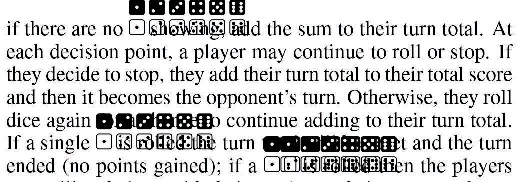
\includegraphics[width=0.9\columnwidth]{figure1} % Reduce the figure size so that it is slightly narrower than the column. Don't use precise values for figure width.This setup will avoid overfull boxes.
\caption{Using the trim and clip commands produces fragile layers that can result in disasters (like this one from an actual paper) when the color space is corrected or the PDF combined with others for the final proceedings. Crop your figures properly in a graphics program -- not in LaTeX.}
\label{fig1}
\end{figure}

\begin{figure*}[t]
\centering
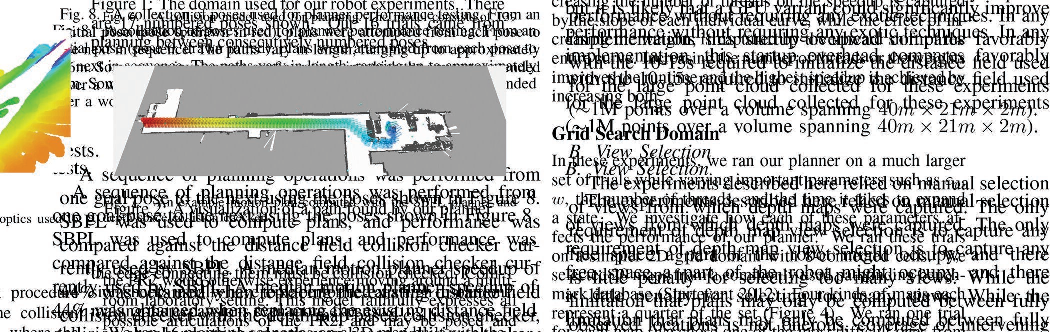
\includegraphics[width=0.8\textwidth]{figure2} % Reduce the figure size so that it is slightly narrower than the column.
\caption{Adjusting the bounding box instead of actually removing the unwanted data resulted multiple layers in this paper. It also needlessly increased the PDF size. In this case, the size of the unwanted layer doubled the paper's size, and produced the following surprising results in final production. Crop your figures properly in a graphics program. Don't just alter the bounding box.}
\label{fig2}
\end{figure*}

% Using the \centering command instead of \begin{center} ... \end{center} will save space
% Positioning your figure at the top of the page will save space and make the paper more readable
% Using 0.95\columnwidth in conjunction with the


Your paper must compile in PDF\LaTeX{}. Consequently, all your figures must be .jpg, .png, or .pdf. You may not use the .gif (the resolution is too low), .ps, or .eps file format for your figures.

Figures, drawings, tables, and photographs should be placed throughout the paper on the page (or the subsequent page) where they are first discussed. Do not group them together at the end of the paper. If placed at the top of the paper, illustrations may run across both columns. Figures must not invade the top, bottom, or side margin areas. Figures must be inserted using the \textbackslash usepackage\{graphicx\}. Number figures sequentially, for example, figure 1, and so on. Do not use minipage to group figures.

If you normally create your figures using pgfplots, please create the figures first, and then import them as pdfs with proper bounding boxes, as the bounding and trim boxes created by pfgplots are fragile and not valid.

When you include your figures, you must crop them \textbf{outside} of \LaTeX{}. The command \textbackslash includegraphics*[clip=true, viewport 0 0 10 10]{...} might result in a PDF that looks great, but the image is \textbf{not really cropped.} The full image can reappear (and obscure whatever it is overlapping) when page numbers are applied or color space is standardized. Figures \ref{fig1}, and \ref{fig2} display some unwanted results that often occur.

If your paper includes illustrations that are not compatible with PDF\TeX{} (such as .eps or .ps documents), you will need to convert them. The epstopdf package will usually work for eps files. You will need to convert your ps files to PDF in either case.

\subsubsection {Figure Captions.}The illustration number and caption must appear \textit{under} the illustration. Labels and other text with the actual illustration must be at least nine-point type. However, the font and size of figure captions must be 10 point roman. Do not make them smaller, bold, or italic. (Individual words may be italicized if the context requires differentiation.)

\subsection{Tables}

\subsection{Tables}

Tables should be presented in 10 point roman type. If necessary, they may be altered to 9 point type. You must not use \texttt{\textbackslash resizebox} or other commands that resize the entire table to make it smaller, because you can't control the final font size this way.
If your table is too large you can use \texttt{\textbackslash setlength\{\textbackslash tabcolsep\}\{1mm\}} to compress the columns a bit or you can adapt the content (e.g.: reduce the decimal precision when presenting numbers, use shortened column titles, make some column duble-line to get it narrower).

Tables that do not fit in a single column must be placed across double columns. If your table won't fit within the margins even when spanning both columns and using the above techniques, you must split it in two separate tables.

\subsubsection {Table Captions.} The number and caption for your table must appear \textit{under} (not above) the table.  Additionally, the font and size of table captions must be 10 point roman and must be placed beneath the figure. Do not make them smaller, bold, or italic. (Individual words may be italicized if the context requires differentiation.)



\subsubsection{Low-Resolution Bitmaps.}
You may not use low-resolution (such as 72 dpi) screen-dumps and GIF files---these files contain so few pixels that they are always blurry, and illegible when printed. If they are color, they will become an indecipherable mess when converted to black and white. This is always the case with gif files, which should never be used. The resolution of screen dumps can be increased by reducing the print size of the original file while retaining the same number of pixels. You can also enlarge files by manipulating them in software such as PhotoShop. Your figures should be 300 dpi when incorporated into your document.

\subsubsection{\LaTeX{} Overflow.}
\LaTeX{} users please beware: \LaTeX{} will sometimes put portions of the figure or table or an equation in the margin. If this happens, you need to make the figure or table span both columns. If absolutely necessary, you may reduce the figure, or reformat the equation, or reconfigure the table.{ \bf Check your log file!} You must fix any overflow into the margin (that means no overfull boxes in \LaTeX{}). \textbf{Nothing is permitted to intrude into the margin or gutter.}


\subsubsection{Using Color.}
Use of color is restricted to figures only. It must be WACG 2.0 compliant. (That is, the contrast ratio must be greater than 4.5:1 no matter the font size.) It must be CMYK, NOT RGB. It may never be used for any portion of the text of your paper. The archival version of your paper will be printed in black and white and grayscale. The web version must be readable by persons with disabilities. Consequently, because conversion to grayscale can cause undesirable effects (red changes to black, yellow can disappear, and so forth), we strongly suggest you avoid placing color figures in your document. If you do include color figures, you must (1) use the CMYK (not RGB) colorspace and (2) be mindful of readers who may happen to have trouble distinguishing colors. Your paper must be decipherable without using color for distinction.

\subsubsection{Drawings.}
We suggest you use computer drawing software (such as Adobe Illustrator or, (if unavoidable), the drawing tools in Microsoft Word) to create your illustrations. Do not use Microsoft Publisher. These illustrations will look best if all line widths are uniform (half- to two-point in size), and you do not create labels over shaded areas. Shading should be 133 lines per inch if possible. Use Times Roman or Helvetica for all figure call-outs. \textbf{Do not use hairline width lines} --- be sure that the stroke width of all lines is at least .5 pt. Zero point lines will print on a laser printer, but will completely disappear on the high-resolution devices used by our printers.

\subsubsection{Photographs and Images.}
Photographs and other images should be in grayscale (color photographs will not reproduce well; for example, red tones will reproduce as black, yellow may turn to white, and so forth) and set to a minimum of 300 dpi. Do not prescreen images.

\subsubsection{Resizing Graphics.}
Resize your graphics \textbf{before} you include them with LaTeX. You may \textbf{not} use trim or clip options as part of your \textbackslash includegraphics command. Resize the media box of your PDF using a graphics program instead.

\subsubsection{Fonts in Your Illustrations.}
You must embed all fonts in your graphics before including them in your LaTeX document.

\subsubsection{Algorithms.}
Algorithms and/or programs are a special kind of figures. Like all illustrations, they should appear floated to the top (preferably) or bottom of the page. However, their caption should appear in the header, left-justified and enclosed between horizontal lines, as shown in Algorithm~\ref{alg:algorithm}. The algorithm body should be terminated with another horizontal line. It is up to the authors to decide whether to show line numbers or not, how to format comments, etc.

In \LaTeX{} algorithms may be typeset using the {\tt algorithm} and {\tt algorithmic} packages, but you can also use one of the many other packages for the task.

\begin{algorithm}[tb]
\caption{Example algorithm}
\label{alg:algorithm}
\textbf{Input}: Your algorithm's input\\
\textbf{Parameter}: Optional list of parameters\\
\textbf{Output}: Your algorithm's output
\begin{algorithmic}[1] %[1] enables line numbers
\STATE Let $t=0$.
\WHILE{condition}
\STATE Do some action.
\IF {conditional}
\STATE Perform task A.
\ELSE
\STATE Perform task B.
\ENDIF
\ENDWHILE
\STATE \textbf{return} solution
\end{algorithmic}
\end{algorithm}

\subsubsection{Listings.}
Listings are much like algorithms and programs. They should also appear floated to the top (preferably) or bottom of the page. Listing captions should appear in the header, left-justified and enclosed between horizontal lines as shown in Listing~\ref{lst:listing}. Terminate the body with another horizontal line and avoid any background color. Line numbers, if included, must appear within the text column.

\begin{listing}[tb]%
\caption{Example listing {\tt quicksort.hs}}%
\label{lst:listing}%
\begin{lstlisting}[language=Haskell]
quicksort :: Ord a => [a] -> [a]
quicksort []     = []
quicksort (p:xs) = (quicksort lesser) ++ [p] ++ (quicksort greater)
	where
		lesser  = filter (< p) xs
		greater = filter (>= p) xs
\end{lstlisting}
\end{listing}

\subsection{References}
The AAAI style includes a set of definitions for use in formatting references with BibTeX. These definitions make the bibliography style fairly close to the ones  specified in the Reference Examples appendix below. To use these definitions, you also need the BibTeX style file ``aaai2026.bst," available in the AAAI Author Kit on the AAAI web site. Then, at the end of your paper but before \textbackslash end{document}, you need to put the following lines:

\begin{quote}
\begin{small}
\textbackslash bibliography\{bibfile1,bibfile2,...\}
\end{small}
\end{quote}

Please note that the aaai2026.sty class already sets the bibliographystyle for you, so you do not have to place any \textbackslash bibliographystyle command in the document yourselves. The aaai2026.sty file is incompatible with the hyperref and navigator packages. If you use either, your references will be garbled and your paper will be returned to you.

References may be the same size as surrounding text.
However, in this section (only), you may reduce the size to {\em \textbackslash small} (9pt) if your paper exceeds the allowable number of pages. Making it any smaller than 9 point with 10 point linespacing, however, is not allowed.

The list of files in the \textbackslash bibliography command should be the names of your BibTeX source files (that is, the .bib files referenced in your paper).

The following commands are available for your use in citing references:
\begin{quote}
{\em \textbackslash cite:} Cites the given reference(s) with a full citation. This appears as ``(Author Year)'' for one reference, or ``(Author Year; Author Year)'' for multiple references.\smallskip\\
{\em \textbackslash shortcite:} Cites the given reference(s) with just the year. This appears as ``(Year)'' for one reference, or ``(Year; Year)'' for multiple references.\smallskip\\
{\em \textbackslash citeauthor:} Cites the given reference(s) with just the author name(s) and no parentheses.\smallskip\\
{\em \textbackslash citeyear:} Cites the given reference(s) with just the date(s) and no parentheses.
\end{quote}
You may also use any of the \emph{natbib} citation commands.


\section{Proofreading Your PDF}
Please check all the pages of your PDF file. The most commonly forgotten element is the acknowledgements --- especially the correct grant number. Authors also commonly forget to add the metadata to the source, use the wrong reference style file, or don't follow the capitalization rules or comma placement for their author-title information properly. A final common problem is text (expecially equations) that runs into the margin. You will need to fix these common errors before submitting your file.

\section{Improperly Formatted Files }
In the past, AAAI has corrected improperly formatted files submitted by the authors. Unfortunately, this has become an increasingly burdensome expense that we can no longer absorb). Consequently, if your file is improperly formatted, it will be returned to you for correction.

\section{Naming Your Electronic File}
We require that you name your \LaTeX{} source file with the last name (family name) of the first author so that it can easily be differentiated from other submissions. Complete file-naming instructions will be provided to you in the submission instructions.

\section{Submitting Your Electronic Files to AAAI}
Instructions on paper submittal will be provided to you in your acceptance letter.

\section{Inquiries}
If you have any questions about the preparation or submission of your paper as instructed in this document, please contact AAAI Press at the address given below. If you have technical questions about implementation of the aaai style file, please contact an expert at your site. We do not provide technical support for \LaTeX{} or any other software package. To avoid problems, please keep your paper simple, and do not incorporate complicated macros and style files.

\begin{quote}
\noindent AAAI Press\\
1101 Pennsylvania Ave, NW Suite 300\\
Washington, DC 20004 USA\\
\textit{Telephone:} 1-202-360-4062\\
\textit{E-mail:} See the submission instructions for your particular conference or event.
\end{quote}

\section{Additional Resources}
\LaTeX{} is a difficult program to master. If you've used that software, and this document didn't help or some items were not explained clearly, we recommend you read Michael Shell's excellent document (testflow doc.txt V1.0a 2002/08/13) about obtaining correct PS/PDF output on \LaTeX{} systems. (It was written for another purpose, but it has general application as well). It is available at www.ctan.org in the tex-archive.

\appendix
\section{Reference Examples}
\label{sec:reference_examples}

\nobibliography*
Formatted bibliographies should look like the following examples. You should use BibTeX to generate the references. Missing fields are unacceptable when compiling references, and usually indicate that you are using the wrong type of entry (BibTeX class).

\paragraph{Book with multiple authors~\nocite{em:86}} Use the \texttt{@book} class.\\[.2em]
\bibentry{em:86}.

\paragraph{Journal and magazine articles~\nocite{r:80, hcr:83}} Use the \texttt{@article} class.\\[.2em]
\bibentry{r:80}.\\[.2em]
\bibentry{hcr:83}.

\paragraph{Proceedings paper published by a society, press or publisher~\nocite{c:83, c:84}} Use the \texttt{@inproceedings} class. You may abbreviate the \emph{booktitle} field, but make sure that the conference edition is clear.\\[.2em]
\bibentry{c:84}.\\[.2em]
\bibentry{c:83}.

\paragraph{University technical report~\nocite{r:86}} Use the \texttt{@techreport} class.\\[.2em]
\bibentry{r:86}.

\paragraph{Dissertation or thesis~\nocite{c:79}} Use the \texttt{@phdthesis} class.\\[.2em]
\bibentry{c:79}.

\paragraph{Forthcoming publication~\nocite{c:21}} Use the \texttt{@misc} class with a \texttt{note="Forthcoming"} annotation.
\begin{quote}
\begin{footnotesize}
\begin{verbatim}
@misc(key,
  [...]
  note="Forthcoming",
)
\end{verbatim}
\end{footnotesize}
\end{quote}
\bibentry{c:21}.

\paragraph{ArXiv paper~\nocite{c:22}} Fetch the BibTeX entry from the "Export Bibtex Citation" link in the arXiv website. Notice it uses the \texttt{@misc} class instead of the \texttt{@article} one, and that it includes the \texttt{eprint} and \texttt{archivePrefix} keys.
\begin{quote}
\begin{footnotesize}
\begin{verbatim}
@misc(key,
  [...]
  eprint="xxxx.yyyy",
  archivePrefix="arXiv",
)
\end{verbatim}
\end{footnotesize}
\end{quote}
\bibentry{c:22}.

\paragraph{Website or online resource~\nocite{c:23}} Use the \texttt{@misc} class. Add the url in the \texttt{howpublished} field and the date of access in the \texttt{note} field:
\begin{quote}
\begin{footnotesize}
\begin{verbatim}
@misc(key,
  [...]
  howpublished="\url{http://...}",
  note="Accessed: YYYY-mm-dd",
)
\end{verbatim}
\end{footnotesize}
\end{quote}
\bibentry{c:23}.

\vspace{.2em}
For the most up to date version of the AAAI reference style, please consult the \textit{AI Magazine} Author Guidelines at \url{https://aaai.org/ojs/index.php/aimagazine/about/submissions#authorGuidelines}

\section{Acknowledgments}
AAAI is especially grateful to Peter Patel Schneider for his work in implementing the original aaai.sty file, liberally using the ideas of other style hackers, including Barbara Beeton. We also acknowledge with thanks the work of George Ferguson for his guide to using the style and BibTeX files --- which has been incorporated into this document --- and Hans Guesgen, who provided several timely modifications, as well as the many others who have, from time to time, sent in suggestions on improvements to the AAAI style. We are especially grateful to Francisco Cruz, Marc Pujol-Gonzalez, and Mico Loretan for the improvements to the Bib\TeX{} and \LaTeX{} files made in 2020.

The preparation of the \LaTeX{} and Bib\TeX{} files that implement these instructions was supported by Schlumberger Palo Alto Research, AT\&T Bell Laboratories, Morgan Kaufmann Publishers, The Live Oak Press, LLC, and AAAI Press. Bibliography style changes were added by Sunil Issar. \verb+\+pubnote was added by J. Scott Penberthy. George Ferguson added support for printing the AAAI copyright slug. Additional changes to aaai2026.sty and aaai2026.bst have been made by Francisco Cruz and Marc Pujol-Gonzalez.

\bigskip
\noindent Thank you for reading these instructions carefully. We look forward to receiving your electronic files!

\bibliography{aaai2026}

\end{document}
